\section{Simulation Results}
The main results of this project will be in the areas concerning the effect of the topology of the lattice on a single island and string collisions.  Variations of these experiments were performed by modifying islands to be more likely to flip, modifying islands by manually flipping them and changing the direction and strength of the magnetic field.
\subsection{Singular Island Experiments}
This experiment, dubbed the sandwich test, was run without any manipulation and roughly 25 evenly spaced `A' islands on the lattice were placed under observation.  The external field was steadily increased to see what value the islands of interest flipped at (if they flipped at all) and these values were recorded.  The external magnetic field applied was incident left to right.
\par
\begin{figure}[ht!]
    \begin{center}
        \subfloat[Initial modified island A sandwich run state][Initial modified island A sandwich run state]{
        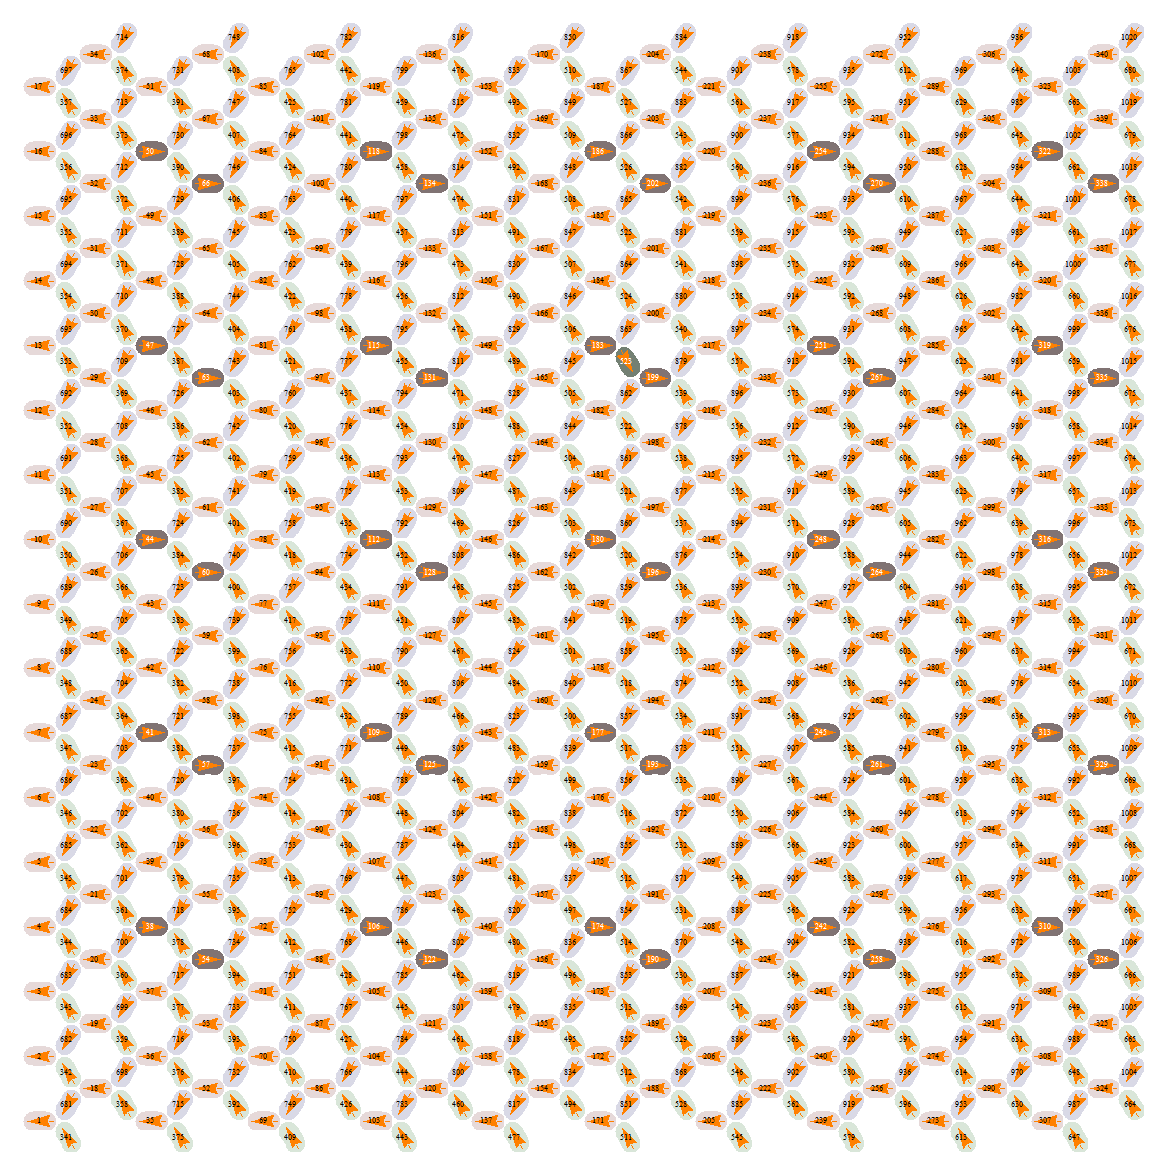
\includegraphics[width=0.45\textwidth]{singislflips.png}
        \label{fig:sf11.1}}
\qquad
        \subfloat[Final modified island A sandwich run state][Final modified island A sandwich run state]{
        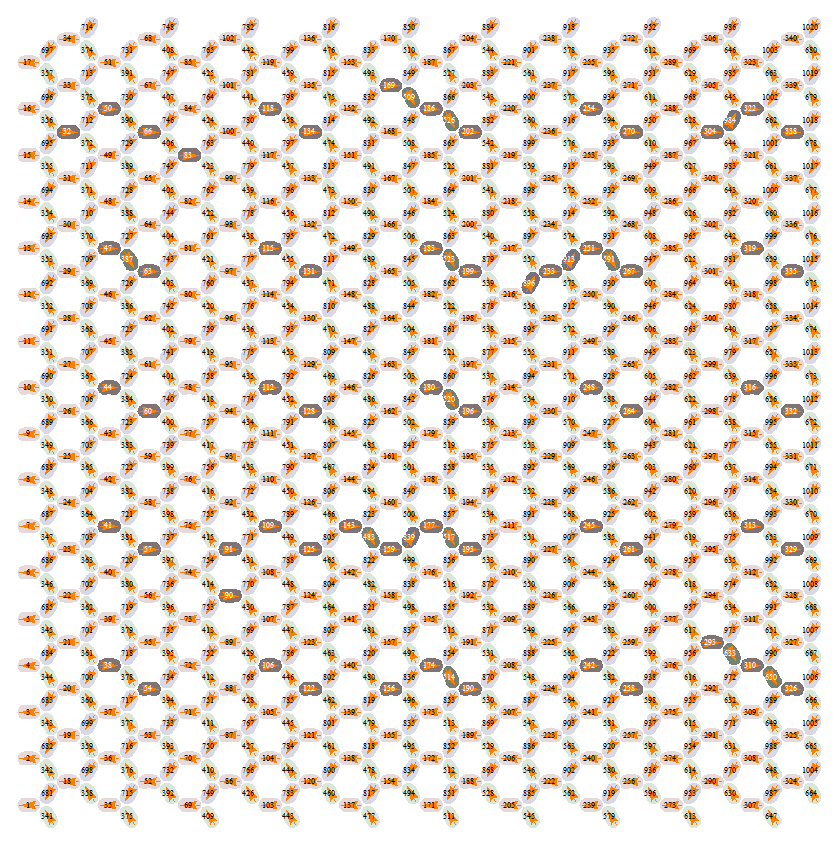
\includegraphics[width=0.45\textwidth]{sandislfinal.png}
        \label{fig:sf11.2}}
        \caption[Modified island A sandwich run states]{Modified island A sandwich run states}
        \label{fig:gf11}
    \end{center}
\end{figure}
Then the lattice was reset and islands sandwiching the islands of interest (hereafter known as sandwich islands) had their anisotropy modified so that they were guaranteed to flip at very low field values.  The experiment was then rerun to see if this had an affect on the flipping of the islands of interest.  One such run can be seen above in figure 12.
\par
The results of all runs of this particular experiment are categorized as follows: Islands which previously did not flip and islands which flipped at lower values.  Some notes on gathering data as the lower the variance is set the greater the number of islands that flip around the same input magnetic field value.  Yet the larger the variance the more likely that islands we are not interested in will perturb results.
\clearpage
For these experiments the variance was kept to $\pm 0.13$ around the average. The field incidence angle was kept to 0 so A islands felt the full weight of the magnetic field to increase the possibility of recording islands flipping.
\par
The key findings for the sandwiched A islands from this was that the roughly 30 \% (with a variance of 22 \%) of islands of interest flipped on each pass and all islands which were flipped in the initial scanning run were flipped at earlier field values.
\par
\begin{figure}[ht!]
    \begin{center}
        \subfloat[Initial modified island B sandwich run state][Initial modified island B sandwich run state]{
        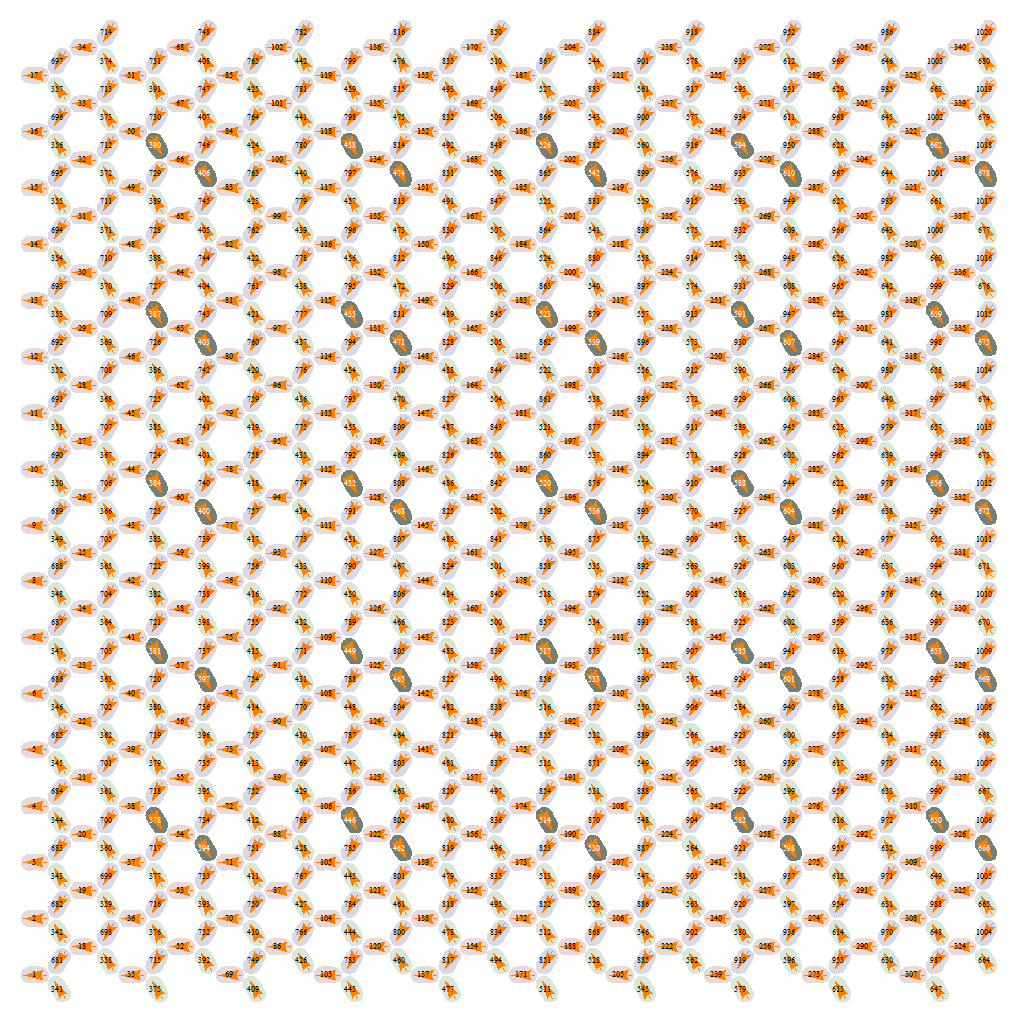
\includegraphics[width=0.45\textwidth]{asandislinit.png}
        \label{fig:sf12.1}}
\qquad
        \subfloat[Final modified island B sandwich run state][Final modified island B andwich run state]{
        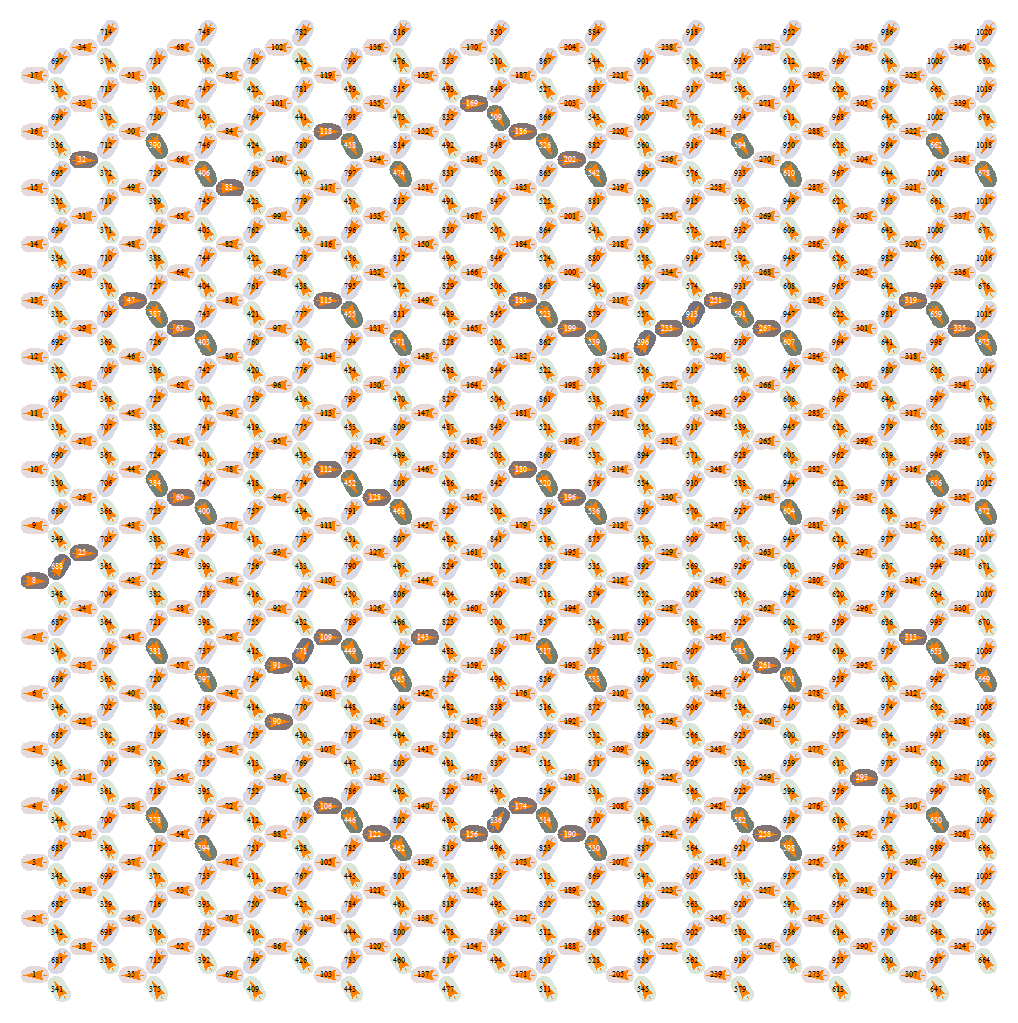
\includegraphics[width=0.45\textwidth]{asandislfinal.png}
        \label{fig:sf12.2}}
        \caption[Modified island B sandwich run states]{Modified island B sandwich run states}
        \label{fi g:gf12}
    \end{center}
\end{figure}
When the field was unbiased these numbers dropped to 16 \% (with a variance of 12\%) islands of interest that flipped.  There is a high variance due to the size of dataset.  If significant statistics were attained this value and it's variance would be more normalized.  The increase in the number of flips when the anisotropy is modified is evidence that by changing the topology of the lattice, neighbouring islands can be softened or flipped easier. Similar experiments could be run on the other `B' and `C' islands but those results would have an equivalent A island analogue by simply changing the angle of incidence of the external magnetic field. A sample run is included above though for completeness.
\par
\subsection{String Collisions}
The second part I have been able to investigate was the impact of string collisions.  Several strings were embedded into the lattice in different forms to see how the strings would interact with each other.
\par
A string was embedded aligning with the external magnetic field.  The strings were generally seperated by a single unflipped island.  From the data of all simulations it was found that you can increase the islands anisotropy by on average 22 \% and it will still flip.  This is direct evidence of the emergence of properties of vertex having an influence on islands contained by them.
\clearpage
\begin{figure}[ht!]
    \begin{center}
        \subfloat[Initial modified A string collision][Initial modified A island string collision]{
        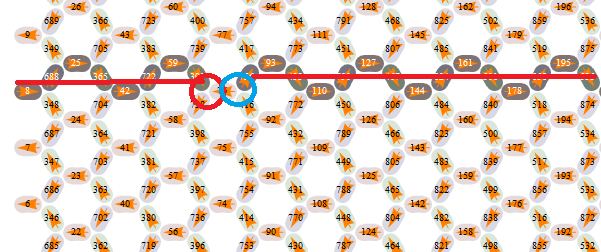
\includegraphics[width=0.4\textwidth]{collisioninit.png}
        \label{fig:sf13.1}}
\qquad
        \subfloat[Final modified sandwich island A run state][Final modified sandwich island A run state]{
        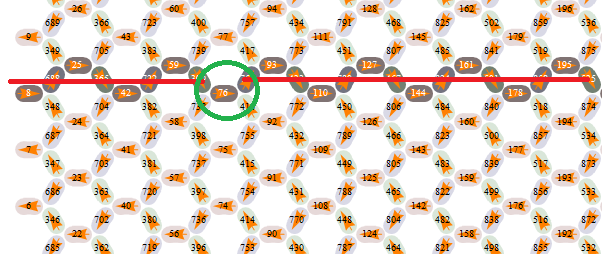
\includegraphics[width=0.4\textwidth]{collisionfinal.png}
        \label{fig:sf13.2}}
        \caption[Modified sandwich island A run states]{Modified sandwich island A run states}
        \label{fig:gf13}
    \end{center}
\end{figure}
In figure 14 we can see two string with opposing monopoles ending beside each other red cirlce is the +q monopole and the blue is marked as the - q Monopole.  The attraction between these two monopoles is such that increasing the anisotropy still results in site 76 flipping.  in this particular case site 76 could have it's anisotropy increased by 17 \% and the island would still flip.
\par
\subsection{Unbiased Magnetic Field}
\begin{figure}[ht!]
    \begin{center}
        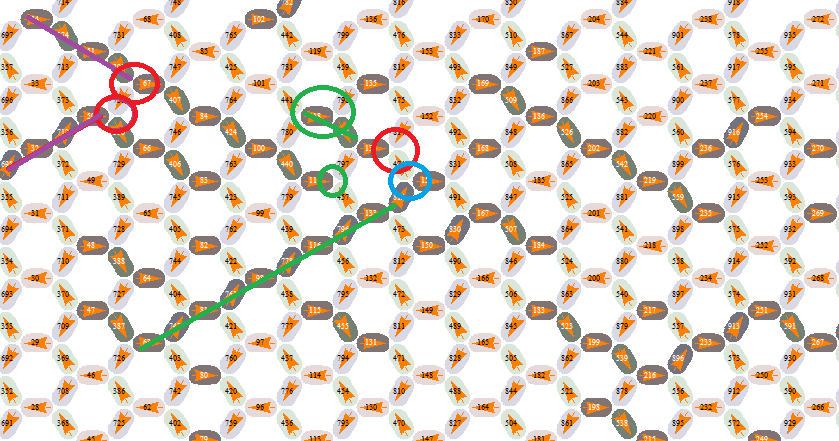
\includegraphics[width=0.8\textwidth]{candidcollide.png}
        \caption[Island flip run]{Unbiased magnetic field.}
        \label{fig:gf14}
    \end{center}
\end{figure}
In addition to the two experiments outlined the last and most interesting experiment was to unbias the field and let some strings form as seen in above figure 15.  The general rules obtained from the few simulations of this nature that were run was that positive monopoles preferred to travel in the same direction the field pointed and that negatively charge poles preferred to move in the opposite directions.  The above figure 15 shows two independent interacting string pairs which formed in the lattice.
\par
The green and purple markings here are the initial flipped islands and strings.  If we look at the purple strings we can see at some stage in the simulation these two positively charged monopoles approached each other and repelled each other by some kind of Coulomb magnetic interaction.  If we observe the green strings they have all converged onto each other.  There is a possibility of the red and blue circled points to collide thus cancelling the monopoles present.
\clearpage
